%!TEX root = ../main.tex
%%%%%%%%%%%%%%%%%%%%%%%%%%%%%%%%%%
% Links:
%
% Difficulty: Companies: 
%%%%%%%%%%%%%%%%%%%%%%%%%%%%%%%%%%

\chapter{Sudoku}
\label{ch:sudoku}
\section*{Introduction}
The game of \textit{Sudoku}\footnote{The literal meaning of "Su-doku" in Japanese is "the number
that is single".} has gained extreme popularity during the last 20 years or so, at the level there
are countless websites and magazines dedicated to it. It is a mathematical-logic-based
number-placement puzzle game where the objective is to fill a nine-by-nine (9x9) grid (subdivided in
$3\times3$ subgrids) with digits so that each:
\begin{itemize}[a)]
	\item \textbf{row},
	\item \textbf{column},
	\item $3\times3$ \textbf{subsquare section}
\end{itemize}
contain number between $1$ and $9$, with the constraint that each number can appear only once in
each section. The puzzle is given as a incomplete grid where only some of the cells are filled (See
Figure \ref{fig:sudoku:example}). This chapter describes how to write a very basic and simple sudoku
solver based on backtracking that can be implemented fast enough during a programming interview.
Having played this puzzle before might help during the interview but it is not fundamental because
the puzzle is easy enough to understand.

\begin{figure}
	\label{fig:sudoku:example}
	\centering
	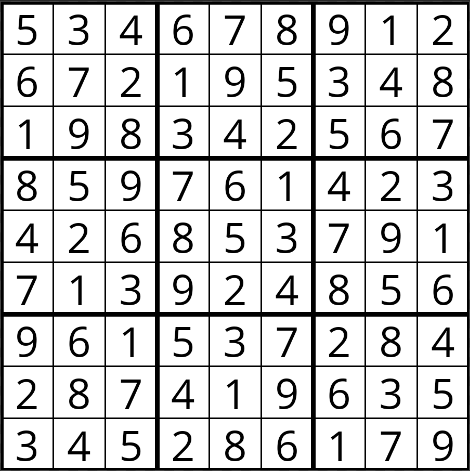
\includegraphics[width=\textwidth]{sources/sudoku/images/sudoku-example}
	\caption{Example of solved sudoku.}
\end{figure}

\section{Problem statement}
\begin{exercise}
Write a function that takes as an input a sudoku grid and returns its solution. The input sudoku
grid is given as a string of lenght $81$ representing the grid in a row-major manner\footnote{In
row-major order, the rows of the grid are stored next to each other in the string.} where empty
cells are represented by the character '0'.
\end{exercise}


\begin{example}
	\hfill \\
	Given the input string
	\tiny{\texttt{"000060280709001000860320074900040510007190340003006002002970000300800905500000021"}}
	{\normalsize the function returns}
	{\tiny\texttt{"431567289729481653865329174986243517257198346143756892612975438374812965598634721"}}
	\normalsize. See Table \ref{tab:sudoku:grid_solution} for a 2D-grid representation.
	
	\begin{table}[]
		\centering
		\begin{tabular}{|l|l|}
		\hline
		Input
		& Solution
		\\ \hline
		\texttt{\begin{tabular}[c]{@{}l@{}}0 0 4 3 0 0 2 0 9 \\ 0 0 5 0 0 9 0 0 1 \\ 0 7 0 0 6 0 0 4
		3 \\ 0 0 6 0 0 2 0 8 7 \\ 1 9 0 0 0 7 4 0 0 \\ 0 5 0 0 8 3 0 0 0 \\ 6 0 0 0 0 0 1 0 5 \\ 0 0
		3 5 0 8 6 9 0 \\ 0 4 2 9 1 0 3 0 0\end{tabular}} & \texttt{\begin{tabular}[c]{@{}l@{}}8 6 4
		3 7 1 2 5 9 \\ 3 2 5 8 4 9 7 6 1 \\ 9 7 1 2 6 5 8 4 3 \\ 4 3 6 1 9 2 5 8 7 \\ 1 9 8 6 5 7 4
		3 2 \\ 2 5 7 4 8 3 9 1 6 \\ 6 8 9 7 3 4 1 2 5 \\ 7 1 3 5 2 8 6 9 4 \\ 5 4 2 9 1 6 3 7
		8\end{tabular}} \\ \hline
		\end{tabular}
		\label{tab:sudoku:grid_solution}
		\caption[Example of Sudoku (2D) and its solution.]{Example of 2D grid represented sudoku and its solution.}
		\end{table}
\end{example}


\section{Clarification Questions}

\begin{QandA}
	\item is the input string guaranteed to only contains numeric charaters and be the right size?
	\begin{answered}
		\textit{Yes the string is guaranteed to be encoding a valid sudoku}
	\end{answered}	
\end{QandA}

\section{Discussion}
\label{sudoku:sec:discussion}
The general problem of solving a sudoku (of size $n\times m$) is NP-complete and thus an efficient
(polynomial-time) solution is not yet known. The naive bruteforce algorithm would have to try each
available number across all empty cells and therefore would have a runtime complexity of
$O(N^(N^2))$, where $N$ is size of the Sudoku puzzle. For a classic  $9 \times 9$ puzzle $N = 9$ and
the number of operations required would be at most $2 \times 10^77$ operations to find a solution
which would make this approach pretty-much impractical. In practice the number of operations vary
hugely according to the difficulty of the puzzle itself and especially according to the number of
given clues which in turn limit the options for each empty cell. Clues reduces the number of
possible states the grid can be and in which the rules of the puzzle are not violated. The more
clues the more are those invalid states. An algorithm can take advantage of that and avoid those
states. For example, a 17-clue puzzle with diagonal symmetry is one of the hardest to solve due to
the large number of candidates and branches\footnote{$17$ clues is also the lower bound for having a
puzzle with a unique solution}. 

Backtracking is therefore a good approach to use to solve this problem considering that the problem
has the following characteristics:
\begin{itemize}
	\item potentially large puzzle-states search space
	\item many \textit{invalid} states we can skip visiting
\end{itemize}
For a more detailed explanation of backtracking see \cite{backtracking}.

In a nutshell the solution proposed in this section works by visiting the empty
cells starting from the first one from the lest, filling it in with a feasible
digit i.e. a digit that does not take the grid to an invalid state, and proceed
to do the same thing for every other cell left empty. If at any point for an
empty cell there is no digit it can contain than a backtracking step occurs. The
choice for the previous cell is then changed and the whole process repeats until
either all the empty cells are filled (in this case we have a valid solution) or
there is no more options for the very first cell (in this case the puzzle has no
solution and it is invalid).
A backtracking solution would solve a puzzle by placing the digit '1' in the
first empty cell and checking if it is allowed to be there i.e. no rules are broken. If
there are no violations (checking row, column, and box constraints) then the algorithm advances to
the next cell and places a '1' in the next empty cell. When checking for violations, if it is discovered that
the "1" is not allowed, the value is advanced to "2". If a cell is discovered where none of the 9
digits is allowed, then the algorithm leaves that cell blank and moves back to the previous cell.
The value in that cell is then incremented by one.

Clearly, this method will eventually find a solution if the puzzle is valid
because all possible valid state for the grid will be visited. 

\subsection{Brute-force}
\label{sudoku:sec:bruteforce}

\lstinputlisting[language=c++, caption={Sample Caption},label=list:sudoku]{sources/sudoku/sudoku_solution1.cpp}

